\documentclass{article}
\usepackage[style=authoryear,backend=bibtex]{biblatex}
\usepackage{float}
\usepackage{graphicx}	
\addbibresource{biblio.bib}
\linespread{1.3}
\usepackage{hyperref}
\hypersetup{ colorlinks=true, allcolors=blue }
\usepackage{caption}
\usepackage[margin=0.8in]{geometry}

% Title Page
\title{%
	UTSC Commuting Patterns \& Transit Reliability\\
}
	
\author{
\small
\hspace*{-4.5mm}
	\begin{tabular}{lll}
		\normalsize\textbf{Jeff Allen} & \normalsize\textbf{Nate Wessel} &  \normalsize\textbf{Steven Farber} \\
		Geography & Planning & Human Geography \\
		MA Student & PhD Candidate & Assistant Professor \\
		\url{jeff.allen@utoronto.ca} & \url{nate.wessel@mail.utoronto.ca} & \url{steven.farber@utoronto.ca}
	\end{tabular}
}



\begin{document}
	
\maketitle


\section{Introduction}

	In this study we analyze how public transit facilitates access to the University of Toronto Scarborough (UTSC) campus. 
	Our aim is to provide an overview of which services are most relevant to UTSC commuters; give some idea what transit trips to campus would look like for students, faculty, and staff; and explore potential barriers and challenges to transit use. 
	
	In Section \ref{sec:commute} we use the home locations of UTSC students, faculty, and staff to estimate the transit routes that commuters would most likely take to campus if everyone used transit. 
	These routes are derived from a transport network dataset including current schedule data of transit agencies in the region (e.g. TTC, GO, DRT). 
	We first use this data to generate summary statistics and plots pertaining to trip durations, waiting times, number of transfers, and walking distances. We then use these estimated routes to create an interactive map which highlights critical transit routes and travel corridors. 
	
	In Section \ref{sec:reliability} we take a close look at reliability on the most important TTC services for UTSC commuters: routes 38, 95, and 198. To do this, we make use of a large GPS dataset from the TTC which lets us observe arrival times at each stop over a period of six months. We compare express and local services in terms of speed and travel time variability, and then look at total travel time distributions between UTSC and selected points. 
	Finally, we make some suggestions for strategies the TTC could use to improve service for UTSC commuters. 

	

\section{Commuting Patterns} \label{sec:commute}

	Given the home locations of UTSC staff and students, we estimate the transit routes that commuters are most likely to take to campus. These routes are derived from current schedule data of transit agencies in the region (e.g. TTC, GO, DRT, YRT), as well as a walking network dataset to account for walking to and from transit stops. We first use this data to generate summary statistics and plots pertaining to mean, median, and distributions of trip durations, waiting times, walking times, and number of transfers. We then use these generated routes to create an interactive map which highlights critical transit routes and travel corridors. This map is online at \url{https://sausy-lab.github.io/utsc-transit-study/commuting-patterns/map.html}

	\subsection{Preparing Data}

		Tabular datasets containing the 6-digit postal codes (FSALDU) of UTSC students, staff, and faculty were provided by UTSC administrators. In total, there are 12,907 students, 644 staff, and 399 faculty in this dataset. Of these 13,950 who travel to UTSC, there were 9,069 unique postal codes. Postal codes represent areal units. In preparation for analysis, they needed to be converted into point coordinates (i.e. geocoded) to represent the exact home location of commuters so they could be inputted into routing software. They were converted to point coordinates using the Postal Code Conversion File (PCCF), a dataset produced by Statistics Canada for linking postal code boundaries to other geographies. This data set is circa 2016, and there were a few recently formed postal codes not included in it. These remaining postal codes were geocoded using Google Maps. (Google was not used for geocoding the entire set as they have a limit of 2,500 per day).

		Not all the postal codes provided are used for analysis. We discarded those which are more than 200km from UTSC or were more than 25km from the nearest transit stop. These locations were deemed unreasonable for typical commutes by transit. There is also some uncertainty whether some of these locations pertain to the postal codes of a student's family, rather than their current place of residence. Table \ref{ntable} summarizes the number of students, staff, and faculty who commute to UTSC, as well as the percent of which are omitted for subsequent analysis.

		\begin{table}[H]
			\centering
			\caption{Counts of students, staff, and faculty used in this study}
			\label{ntable}
			\begin{tabular}{l|lll}
	        & n input & n for & Percent \\ 
	        & dataset & analysis & removed \\ \hline
				Students & 12,907        & 12,298          & 4.72\%          \\
				Staff    & 644           & 631             & 2.02\%          \\
				Faculty  & 399           & 392             & 1.75\%          \\
				Total    & 13,950         & 13,321           & 4.51\%         
			\end{tabular}
		\end{table}

		The maps in the appendix (Figures \ref{pt_students} and \ref{pt_stafffaculty}) show the location of the geocoded locations of UTSC students, staff, and faculty. Students are more located in Scarborough and Markham, with particularly high concentrations in higher density areas like Scarborough town centre. Faculty are clustered in the wealthier neighbourhoods closer to downtown Toronto (many are cross-appointed with the downtown St. George campus). UTSC staff, however, are more dispersed among the more middle-class suburban areas surrounding UTSC.

	
	\subsection{Estimating Transit Routes}

		The next step in our analysis was to estimate the trip characteristics from each of these home locations of students, staff, and faculty to UTSC (i.e. for a typical commute). To do so, we built a custom multi-modal network graph for the Toronto region. This network graph allows for computing transit trip itineraries between two or more points. It incorporates time walking to and from stops, waiting for a vehicle, in-vehicle travels times, and any time spent transferring between vehicles. This network graph was built using an open-source routing engine (\cite{otp}). This has two sets of inputs. The first are a network of walking paths, sourced from OpenStreetMap. The second are transit schedules in the form of GTFS (Genreal Transit Feed Specification) data for eleven transit agencies\footnote{This includes data from the Toronto Transit Commission, Durham Regional Transit, GO Transit, York/VIVA, MiWay, Brampton Transit, Oakville Transit, Burlington Transit, Hamilton Street Railway, Barrie Transit, Grand River Transit} that serve the Toronto region. The GTFS and OSM data used for this anlaysis is circa April 2018, the same time period in which the postal code location data was received from UTSC. Similar networks have been used to analyze the travel behaviour of University students in the Toronto region (\cite{allen2018}).

		The routes were estimated by inputting the home coordinates, the coordinates of UTSC, and a departure time into the network graph. The departure time for trips was randomly selected between 8:00am and 11:00am, the time period in which the majority commuters commence their journey. The output includes the transit agencies and route identifiers for the transit portions of the trip (e.g. TTC 198, GO Bus 51, etc.), the total duration of the trip, the time spent walking to and from stops, time spent waiting for a vehicle, and number of transfers required for each trip. These are tabulated, described, and plotted in the following section. The output also includes the geometry of the path taken, which is later used to map and analyze the spatial patterns of where people are commuting from.


	\subsection{Summary Statistics of Trip Attributes}
	
		This section provides a summary of transit commuting for students, staff, and faculty to UTSC. It should be noted that the following analysis is only an estimate as the input data does not include the travel mode in which students typically travel. From two recent travel surveys, 60\% (\cite{smto}) and 53\% (\cite{utsc}) of students commuted by transit. Those who live close by are more likely to walk and bike, while those living further away or live in areas with limited transit provision are more likely to drive. 
		
		Figure \ref{fig:toproutes} displays the top ten most relied upon routes for UTSC faculty, staff, and students. These bars do not total 100\% since many are reliant on more than one route (e.g. they take the subway, then transfer to bus 198). As expected, students are likely to use three TTC routes that provide direct access to UTSC (38, 95, and 198). The 95 in particular has a large share of riders commuting to UTSC. Other than these three TTC routes, students are also likely to take GO Bus 51, which is a regional route connecting UTSC to Pickering, Markham, and Richmond Hill, as well as Scarborough Town Centre. Faculty are much more likely to use the 198 bus, connecting from the Bloor-Danforth subway (Line 2), as most faculty live closer to downtown Toronto. Staff use the expected TTC routes (38, 95, and 198), and are also likely users of bus 900 by Durham Region Transit as a higher proportion of staff live east of UTSC in Durham Region.
		
		Figure \ref{fig:o_durations} shows a summary of the estimated total travel (one-way) for commuting to UTSC. This is the estimated total of all walking, waiting, and in-vehicle portions of a transit trip. Figure \ref{fig:o_walk} displays just the portion of time spent walking on a transit trip. This includes walking from home to a transit stop, any time walking between stops when transferring between vehicles, and walking from the alighting stop to UTSC. These values may be slightly underestimated depending on where their final destination is on UTSC. For example, students who are going to the Pan Am centre my have a longer walk at the end of their trip than students who are going to class in a building closer to the main bus stops (e.g. in the Academic Resource Centre or the Bladen Wing). Figure \ref{fig:o_wait} is the estimated time spent waiting over the course of a transit trip. For example, if a trip incorporates two transit routes, the wait time shown in Figure \ref{fig:o_wait} is the time waiting at the first stop plus any time waiting at the second stop. Lastly, Table \ref{transfers_table} displays the estimated number of transfers required on a one-way transit trip to UTSC. Staff and faculty are more likely to require more transfers than students. 
		
		It should be noted that this analysis is based on the scheduled transit service, and therefore does not account for any unreliability of on-the-ground transit service due to congestion, bus-bunching, or otherwise. More precise analysis of travel times and waiting times  based on the GPS tracked location of vehicles for select set of routes and stops is provided in Section \ref{sec:reliability}. 
		
		
		\begin{figure}[H]
			\caption{Counts and percent of trips for the top 10 transit routes for UTSC commuters}
			\centering
			
			\hspace*{-23mm}
			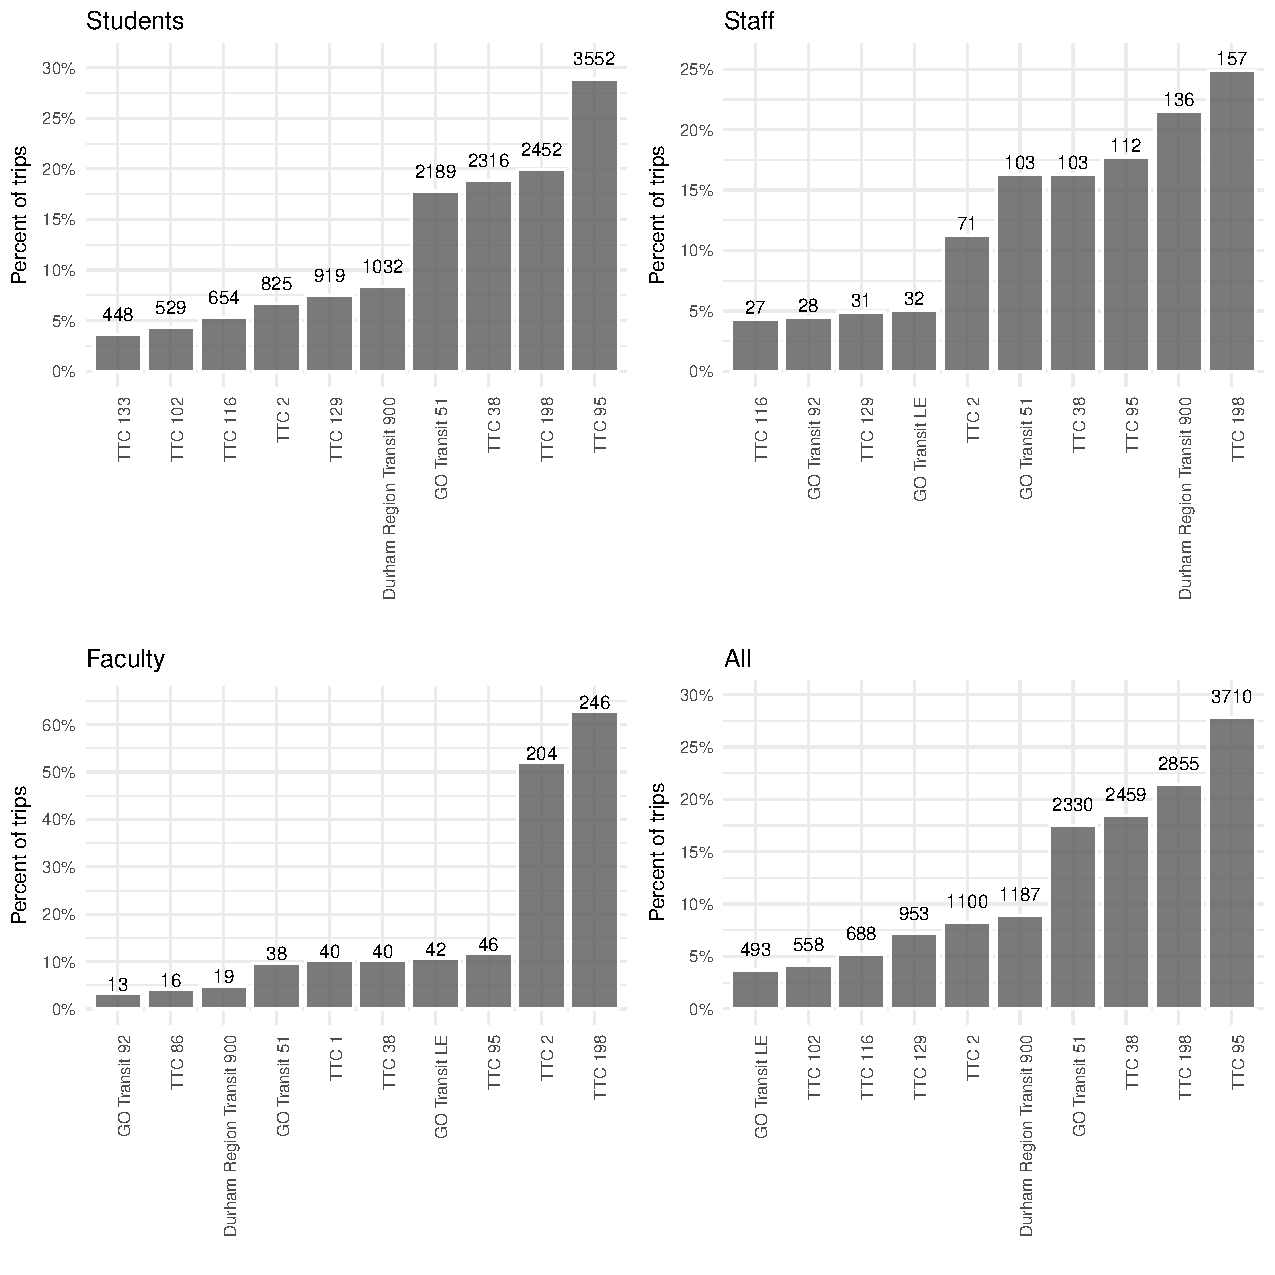
\includegraphics[width=6.5in]{figures/top_routes.pdf}
		%	\caption{blah}
			\label{fig:toproutes}
		\end{figure}
	

		\begin{figure}[H]
			\caption{Summary of total travel time for transit commutes}
			\centering
			
			\hspace*{-23mm}
			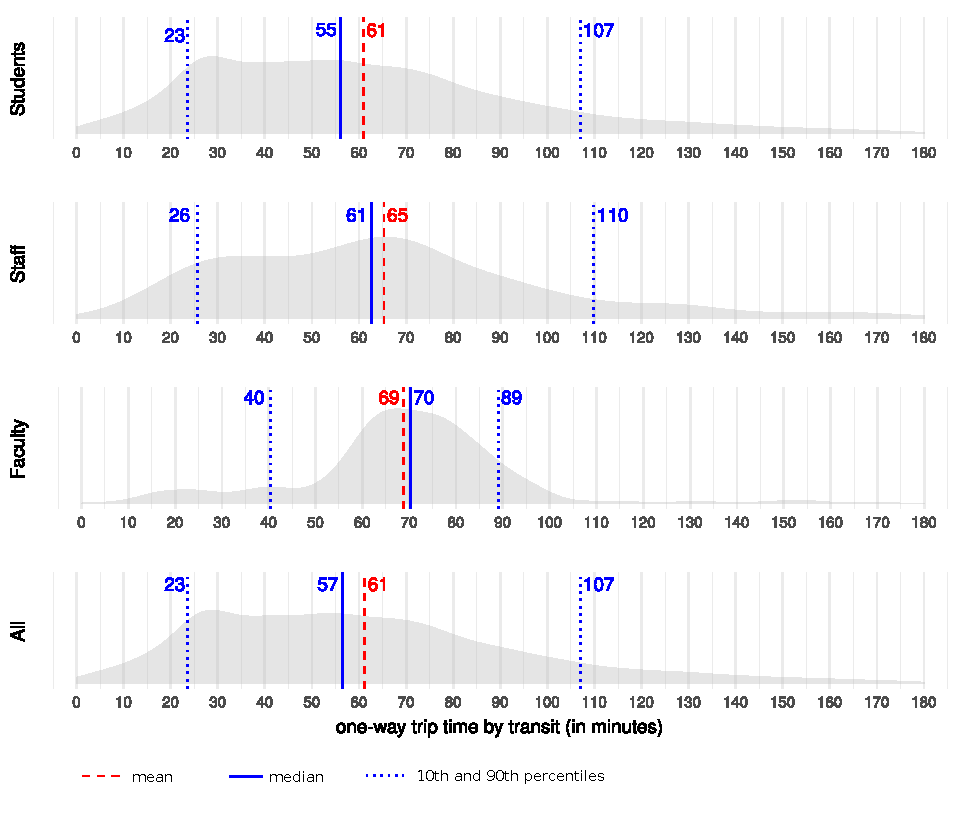
\includegraphics[width=6.5in]{figures/o_duration}
			%	\caption{blah}
			\label{fig:o_durations}
		\end{figure}
	
	
		\begin{figure}[H]
			\caption{Summary of total walking time for transit commutes}
			\centering
			
			\hspace*{-23mm}
			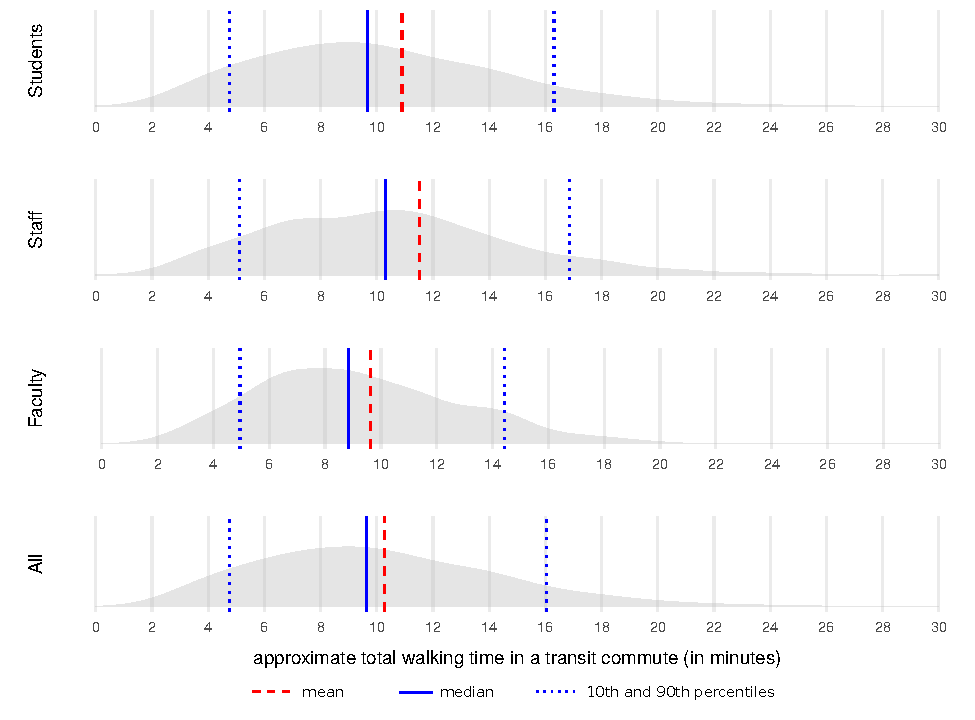
\includegraphics[width=6.5in]{figures/o_walk}
			%	\caption{blah}
			\label{fig:o_walk}
		\end{figure}
	
	
		\begin{figure}[H]
			\caption{Summary of total waiting time for transit commutes}
			\centering
			
			\hspace*{-23mm}
			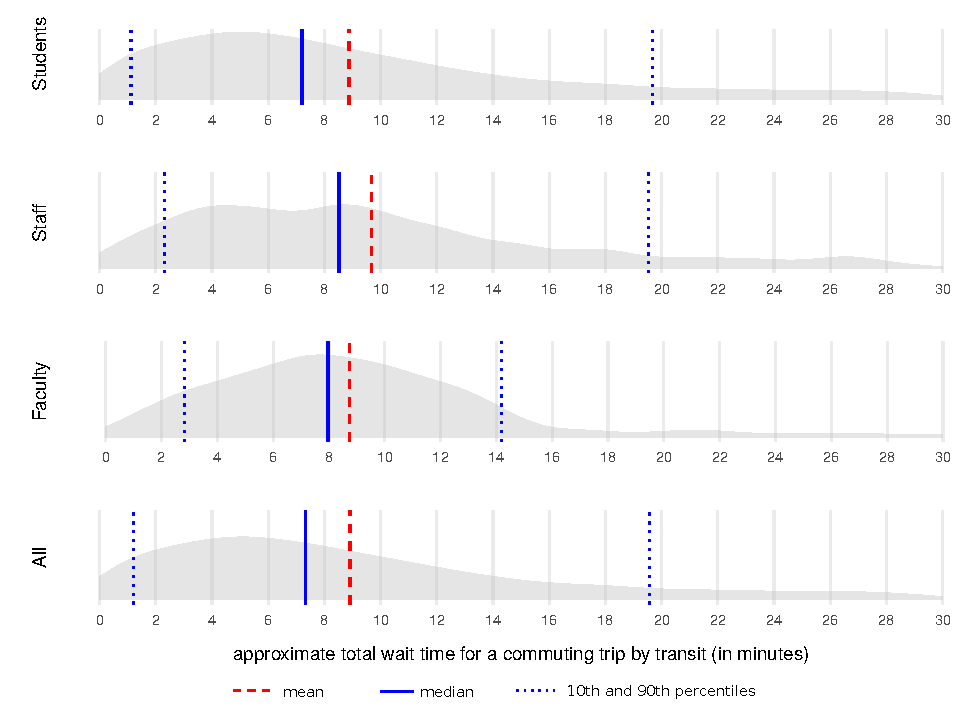
\includegraphics[width=6.5in]{figures/o_wait}
			%	\caption{blah}
			\label{fig:o_wait}
		\end{figure}
	

		\vspace{5mm}
		\begin{table}[H]
			\centering
			\caption{Number of transfers during commutes by transit}
			\label{transfers_table}
			\label{my-label}
			\begin{tabular}{llllll}
				& \multicolumn{5}{c}{Number of Transfers}                            \\
				& 0             & 1             & 2             & 3+          & Mean \\ \hline
				Students & 2758 (22.4\%) & 5566 (45.3\%) & 3275 (26.6\%) & 699 (5.6\%) & 1.17 \\
				Staff    & 109 (17.3\%)  & 304 (48.2\%)  & 184 (29.1\%)  & 34 (5.4\%)  & 1.23 \\
				Faculty  & 29 (7.4\%)    & 189 (48.2\%)  & 149 (38.0\%)  & 25 (6.4\%)  & 1.44 \\
				All      & 2896 (22.4\%) & 6035 (46.7\%) & 3434 (26.6\%) & 552 (4.3\%) & 1.18
			\end{tabular}
		\end{table}
		
		
	\newpage 
		
	\subsection{Interactive Map of Transit Commutes}
		
		We also generated an interactive map to display the spatial patterns of transit commutes to UTSC. This map is designed to highlight where students are commuting from, which are the critical travel corridors, as well as provide comparison between students, staff, and faculty. The map is online at \url{https://sausy-lab.github.io/utsc-transit-study/commuting-patterns/map.html}.
	
		The map was built by overlaying the trips generated in the previous section. Each trip is displayed with a faint transparency, but when overlaid, it highlights the critical travel routes by transit to UTSC. Buttons in the top left of the map allow for switching between maps and data showing only students, staff, or faculty. The maps for faculty and staff show a greater concentration of travel flow than students who are commuting from more dispersed locations. The map can also be rotated or zoomed in and out. For easier display, the geometries of the routes were simplified when zoomed out using an algorithm which limits the number of points along a line segment (\cite{douglas1973}). When zoomed in, the lines become more visible to show where students are travelling from within a neighbourhood context. The background data is from OpenStreetMap.



\section{Transit Reliability}\label{sec:reliability}
	Figure \ref{fig:toproutes} in the previous section identified several important routes for potential transit commuters; of potential transit trips to campus, the schedule-based analysis showed that roughly 25\% would make use of TTC's route 95, 20\% of route 198, and 17\% of route 38.
	In this section we look at the reliability of those lines using a large dataset of GPS recordings from the actual vehicles. 

	The reliability of transit services can be thought of in a lot of different ways. For infrequent services like regional GO buses, adherence to a published schedule may be the most important consideration since people use schedules to time their trips. Most TTC services however are frequent enough, and perhaps variable enough, that checking a schedule isn't much use; people generally figure out about how long their trip will take and just arrive at the stop when they need to travel.\footnote{
		Even if people use a real-time transit app to time their arrival, it's reasonably fair to consider that wherever they wait, they're still waiting for the next vehicle. The time they check the app could then be considered as the time they start waiting.
	} 
	In cases like this we don't use the schedule as a point of departure but instead try to see what trips are like for an average passenger, and especially how predictable those trips are. A reliable high-frequency service is one that has consistent travel times without too many unexpected delays. 

	In the first part (Section \ref{sec:exp_v_loc}) we focus on the express services, route 198 and the 95E, and compare en-route travel time performance to equivalent local services. This should help us understand whether these services are actually able to bypass some of the delays and travel time variability that they are designed to avoid.
	The second part (Section \ref{sec:travel_times}) gives a bit more of a passenger's perspective by adding in average wait times to estimate the total time someone would need to travel between UTSC and various points on the 198, 95 and 38. For route 95, we compare express and local services and whether the express offers an advantage to the average traveller. 

	
	\subsection{Data}
		GPS data for this portion of the study were scraped from the \href{https://www.nextbus.com/xmlFeedDocs/NextBusXMLFeed.pdf}{NextBus API} which provides GPS positions for all active vehicles in TTC's fleet, every 20 seconds, via a web interface. This data is typically used for real-time transit apps, but can be collected and stored for analysis. 
		We used a tool described in Wessel, Allen, \& Farber (\cite*{Wessel2017}) and available \href{https://github.com/SAUSy-Lab/retro-gtfs}{here} for collecting the data and processing it into distinct trips associated with stops and arrival times, similar to the schedule data used in Section \ref{sec:commute}. This format allows us to query the data directly to get travel times at any particular moment between two stops.
		
		The data used for this study spans a bit over six months, from October 21st, 2017 to April 22nd, 2018, except for a three day gap from November 15 - 17 when our server went down temporarily. To keep things simple we'll be looking only at regular weekday service (e.g. not including holidays) which leaves 127 full days of data.
		
		As with any large, complex dataset it's quite possible that it isn't fully representative of actual events in the real world. Specifically, we know some vehicles occasionally report the wrong route, don't have a working transponder, or otherwise produce no data or erroneous data. The TTC actually has very good data in this regard relative to other agencies, and we're confident that the measures shown here are accurate and representative for our purposes. Based on experience working with the data, we estimate that more than 95\% of vehicles are reporting accurate information at any given time. 

	\subsection{Express vs. Local Service}\label{sec:exp_v_loc}
		The first broad question to be addressed is whether express services are actually much faster or more reliable than local services. Express services like the 198 and 95E for the most part only stop at major intersections that connect to other transit lines. Local services by contrast may make one or more intermediate stops between major intersections. The difference can be pretty substantial, with the 95E making 18 stops between its termini while the 95A makes as many as 53 stops over the same course.\footnote{
			Neither line strictly has to make all its stops though, and the local services probably skip many stops regularly because nobody on a given bus needs them.
		}
		Beside increasing speed, making fewer stops should also decrease travel time variability since stop dwell time can be very inconsistent.
		
		We start first with route 198, which runs between Kennedy Station and UTSC making 12 intermediate stops where the route connects to other lines.\footnote{
			Descriptions and links to maps of this and other routes dealt with in this section can be found in the appendix, Section \ref{appendix:route_descriptions}.
		} 
		There is no precise local equivalent of the 198, but for about 75\% of its 10km route it runs parallel to route 86 which serves local stops. To compare the two, we observe the duration of trips on the 198 versus the 86 running on the shared portion of their routes, from Kennedy Station to the intersection of Kingston Road and Lawrence Avenue East. Figure \ref{fig:198_vs_86} shows the distribution of travel times, not including wait times, for vehicles running between those two points, both eastbound and west bound during both morning peak (7 - 9AM) and evening peak (4 - 6PM) service. 

		\begin{figure}[h]
			\centering
			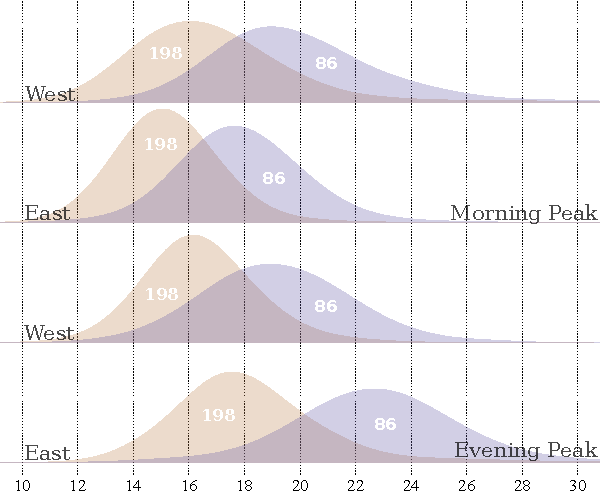
\includegraphics{figures/198_vs_86_kennedy_lawrence}
			\caption{En-route travel time distributions of the 198 (express) versus the 86 (local) between Kennedy station and Lawrence Avenue.}
			\label{fig:198_vs_86}
		\end{figure}

		There is a lot of overlap in the travel time distributions, meaning that the 86 is sometimes faster than the 198 over our six month observation period, but the big picture clearly shows an advantage for the 198 over the 86. The overlap in the distributions is likely due to speed differences between different days for both routes rather than being representative of the travel time distribution of every day in the sample. 
		The difference in median travel times between the two routes ranges from around 2.5 to 5 minutes over the shared portion of the route. 
		If one were to imagine that there were a direct local equivalent of the 198, these time savings could be projected forward over the remaining 2.5km of the route and yield travel time savings of around 3.3 to 6.6 minutes compared to a local service running under the same conditions.
		Figure \ref{fig:198_vs_86} also shows consistently more variable travel times for the local service which can be seen as lower, broader distributions for the 86. 
		
		It's important to note though that the comparison is not quite fair - in the absence of a frequent express service, local-running services like the 86 could be inundated with passengers they don't currently serve and experience crowding and traffic conditions that they don't currently have to deal with. That is, it's quite possible that the presence of the express line actually speeds up service on the local. 
		
		
		Route 95E is the other express line we'll be considering. It runs east-west between UTSC and York Mills Station on York Mills Road and Ellesmere Road. There are two local variants which we can use for comparison, the 95A \& 95B\footnote{
			Again, see Appendix \ref{appendix:route_descriptions} for detailed descriptions and route maps.
		}. 
		As before, we look at bus travel times between two points where the express and local services overlap: Bayview Avenue\footnote{
			Due to the technical difficulty of matching buses to the street network as they access York Mills station via an underground tunnel, we get more reliable results by moving one stop over to Bayview Avenue, which can be used as an approximate western terminus.
		} and UTSC at Ellesmere and Military Trail. Figure \ref{fig:95EvL} shows the travel time distributions for the local and express variants over 16.5km of shared route.

		\begin{figure}[h]
			\centering
			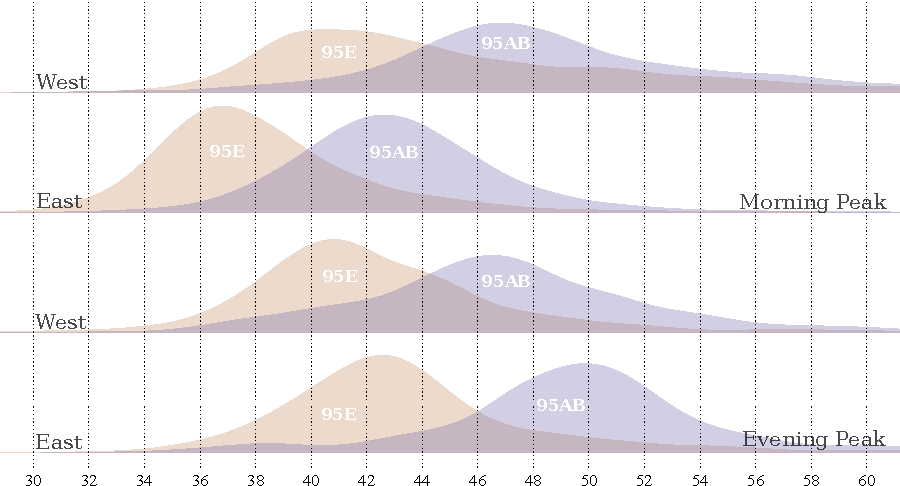
\includegraphics{figures/95_vs_95e_bayview_UTSC}
			\caption{Travel time distributions of the 95E (express) vs. 95A \& 95B (local) between Bayview Avenue and UTSC.}
			\label{fig:95EvL}
		\end{figure}
		
		Again, a definite travel time advantage can be observed for the 95E express service, equal here to about an 8 to 10 minute difference between medians. Any advantage in travel time variability is not so clear; it appears that both express and local services have pretty broad distributions with long tails representing occasional large delays. It's to be expected that the 95 should show more variability than the 198/86 shown in Figure \ref{fig:198_vs_86}; the route analyzed here is roughly twice as long. Still, this fact alone does not seem to explain the difference, statistically at least. En-route travel times are more variable on route 95.
		
		There are some interesting things to note about both figures \ref{fig:198_vs_86} and \ref{fig:95EvL}. 
		First, we can clearly see the effect of rush hour travel patterns on travel times during the peak periods. In Toronto overall, people flow toward the centre of the city in the morning and out again in the evening. For the lines in question this means that eastbound morning service is faster than westbound service and that conversely westbound service is faster in the evening. Given what we saw in Section \ref{sec:commute} about the home locations of UTSC commuters, this may constitute a substantial advantage for the many people who spend the day on campus but live to the west. 
		
		% TODO should I just kill this section since it looks at the commute in the wrong direction?
		Another thing that's noticeable in both plots is the long tail on the distribution for travel times in some periods, especially the westbound morning peak period in both figures and the westbound evening peak period in Figure \ref{fig:95EvL}. 
		These travel time distributions were made by lumping together observed travel times on 127 weekdays; it's quite possible that the long tailed distribution is typical of this period, but not of any particular day.
		The worst case is definitely the westbound morning peak for route 95 in Figure \ref{fig:95EvL}, so to explore this further, we looked more closely at travel times for each service day for westbound local services (95A \& B) in the morning peak.
		
		Indeed, it does seem that several particularly bad days are mostly responsible for the long tail, but it is also interesting to note that the 95A has substantially slower travel times than the 95B through this section. The reason for this is not known. A preliminary analysis wasn't able to identify winter weather as a definite correlate with poor service on particular days. It's possible that the two routes are operated differently in some relevant way by the TTC.

		%		w$direction_id: 95_1_95A
		%		Min. 1st Qu.  Median    Mean 3rd Qu.    Max. 
		%		31.39   41.31   43.76   45.44   47.99   97.11 
		%		------------------------------------------------------------- 
		%		w$direction_id: 95_1_95B
		%		Min. 1st Qu.  Median    Mean 3rd Qu.    Max. 
		%		28.34   36.77   39.29   39.13   41.08   64.32 
		
		
		In summary, it does appear that express services offer a substantial in-vehicle travel time advantage over local services, in the range of a 15 - 21\% time savings for route 198 and 9-14\% for route 95. These statistics however do not include time spent waiting and need to be balanced against the understanding that these express services are less frequent than the equivalent local service; wait times for express buses will therefore tend to be longer.\footnote{
			In rough numbers, the 95E and 198 run only about $\frac{1}{4}$ to $\frac{1}{3}$ as often as the local comparison routes. Route 86, used as a comparison for the 198 does not actually reach campus, but 95A and 95B offer a real alternative.
		} We explore wait times and total travel times to and from UTSC in the following section.

	\subsection{Travel times to and from UTSC}\label{sec:travel_times}
		In this section we look at total travel times, including average wait times, for trips to and from UTSC from selected stops along routes 198, 95 and 38. Since most UTSC commuters live to the west of campus the focus of the discussion will be on eastbound morning and westbound evening service. We should see again in this section that travel in the other direction generally takes longer and is less reliable. 
		In addition, we break out wait times from the total travel time; people generally perceive waiting for a vehicle as more of a burden than in-vehicle travel time \parencite[see e.g.][]{Mishalani2006} so this time can have a disproportionate impact on perceptions of reliability and service quality \parencite{Watkins2011}.
		In line with the previous section we also look closely at express and local alternatives where they are available for routes 95 and 38.
		
		Since service on all three lines is fairly frequent throughout the day, we can assume that people arrive to their stops at essentially random times rather than using a schedule to coordinate their arrival as they might with a less frequent service like GO.
		This assumption greatly simplifies the estimation of average wait times. We sample arrival times over the peak travel periods and take the wait time as the time until the next arriving vehicle. The total travel time then is the time from the start of waiting until arrival at the destination stop. Nothing shown here includes time spent walking to or from transit stops. 
		
		Figure \ref{fig:198_east_morning} shows wait times and total travel times for route 198 eastbound in the morning peak. The westbound evening service is shown in Figure \ref{fig:198_west_evening}. 
		In both figures, the band along the bottom shows the distribution of wait times by giving the 10-90\% inter-decile range; the dashed line shows the median. 
		The upward sloping band shows total travel times for the same range (10, 50, 90\%). 
		
		\begin{figure}[h]
			\centering
			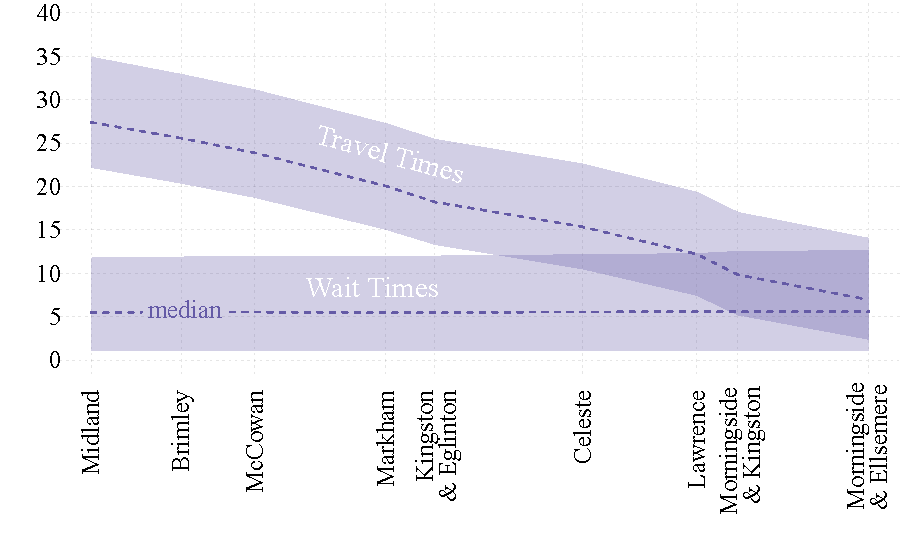
\includegraphics{figures/198_east_morning}
			\caption{ Waiting and travel times (in minutes) from selected stops to UTSC for the 198 eastbound during morning peak service.}
			\label{fig:198_east_morning}
		\end{figure}
		
		\begin{figure}[h]
			\centering
			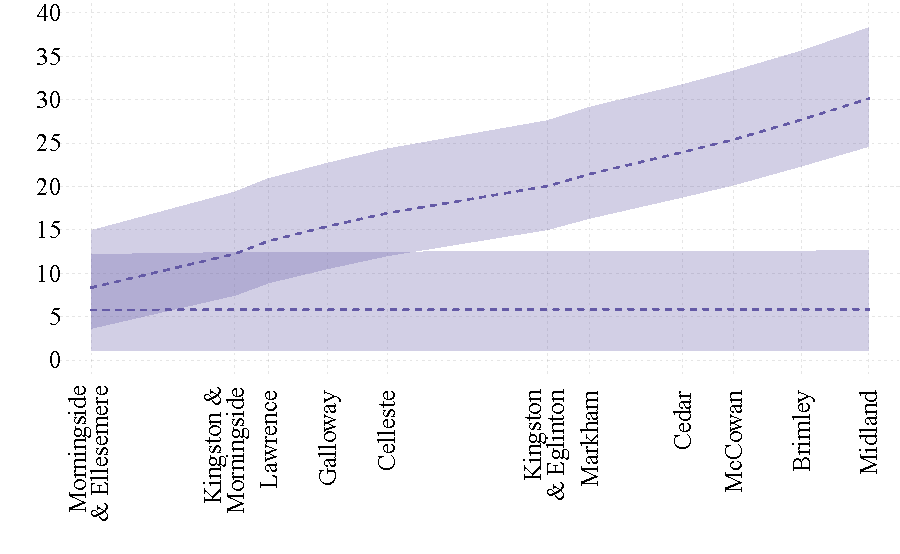
\includegraphics{figures/198_west_evening}
			\caption{ Waiting and travel times (in minutes) from UTSC to selected stops for the 198 westbound during evening peak service.}
			\label{fig:198_west_evening}
		\end{figure}
		
		For trips east toward UTSC, wait times appear to be extraordinarily constant between stops, or constant at least in their variability, with a median of about 6 minutes and an upper bound around 12. Combining this plot with Figure \ref{fig:198_vs_86}, it seems that by far the biggest factor in total travel time variability for this line is the wait time.
		The figure for westbound evening travel is very similar, though with slightly longer waiting and travel times. The wait time in this case is constant since times are all calculated from the same stop at UTSC. 
		
		When the 198 was launched by the TTC several years ago, it advertised 30 minute trips between UTSC and Kennedy Station. It is not clear whether that figure was meant to include time spent waiting, but even if it was, it appears that the 198 is performing about as expected, at least during the peaks in the direction of the reverse commute.
		
		
		Next we turn to routes 95 and 38. Route 38 mostly overlaps with the 95, joining it just past Scarborough Town Centre at Bellamy Drive, which lets us consider the two lines together. And the 95E presents passengers with an interesting choice not available to those on the 198: is it better to wait for an express bus or just to catch the first bus that comes whether it's local or express? 
		Figure \ref{fig:95_east_morn} uses in the same style as Figure \ref{fig:198_east_morning} but adds an express-only alternative to compare the two strategies. Waiting for the express is shown in orange while the any-bus option is shown in purple. 
		
		\begin{figure}[h]
			\centering
			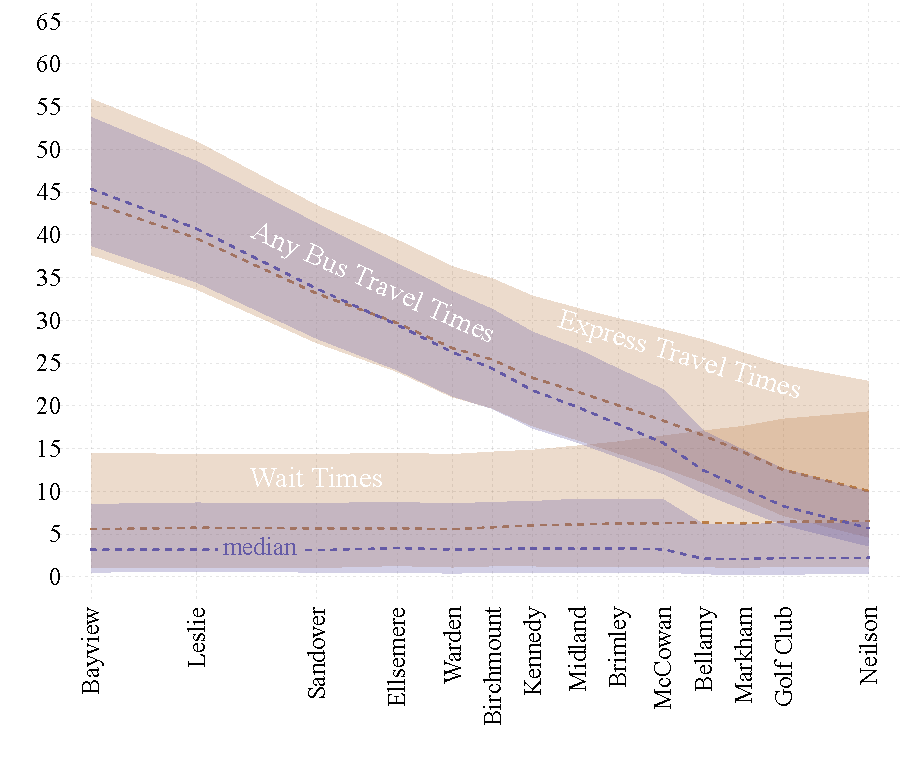
\includegraphics{figures/95_east_morning}
			\caption{ Waiting and travel times for the 95 westbound during morning peak service; Comparison of waiting for the express versus catching the next arrival.}
			\label{fig:95_east_morn}
		\end{figure}
		
		\begin{figure}[h]
			\centering
			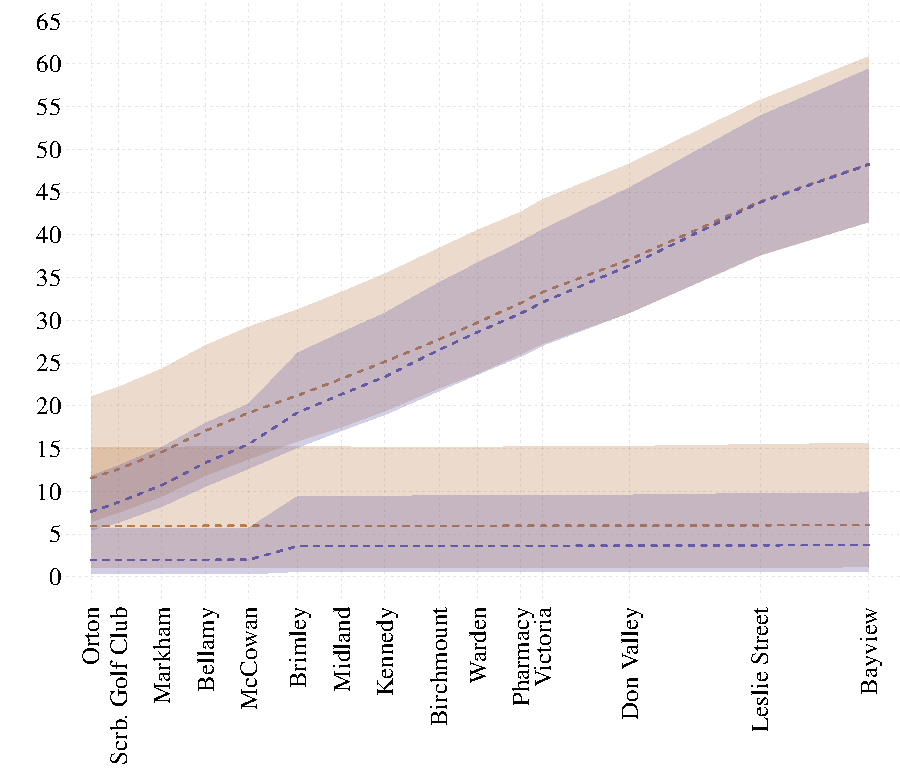
\includegraphics{figures/95_west_evening}
			\caption{ Waiting and travel times for the 95 westbound during evening peak service; Comparison of waiting for the express versus catching the next arrival.}
			\label{fig:95_west_even}
		\end{figure}
		
		There are some interesting things to note in these figures. First, there is a big change in wait times for the any-bus strategy between McCowan and Bellamy roads. This is where the 38 joins the stream of 95 buses, effectively making service to UTSC more frequent from McCowan onward than it was at Brimley. Next, we note that things are changing along the course of this route much more than they were for the 198. The length of route shown here is about twice as long as that of the 198 and reliability tends to degrade on longer routes. Transit agencies often try to evenly space departures at terminal stations, but they are less able to keep vehicles from bunching when they are all moving down the road together, some going faster, some slower. 
		While wait times are pretty constant for the any-bus strategy, travel time variability appears to increase along the length of the route, meaning that much of the variability there is introduced once people have already boarded. 
		The express-only strategy has wait times that are pretty steady between Bayview and Warden, but then start to increase as the line goes on toward UTSC and the express vehicles start to bunch. This appears to account for most of the increase in travel time variability from stops nearer campus.
		
		Naturally enough, the strategy of catching whatever bus comes first yields lower average wait times with a median wait close to 2 or 3 minutes versus about 6 minutes for express-only. For stops close to UTSC, the difference in wait times for these strategies totally outweighs the travel time benefits of express service shown in the previous section. Even at Bayview\footnote{
			As in Section \ref{sec:exp_v_loc} there is some trouble in connecting the 95 with it's underground terminal at York Mills Station, but it seems safe to project the trend lines forward another couple of kilometers and expect that the express-only strategy would marginally outperform the any-bus strategy at the terminal station. 
		}, the benefit of the express service appears to be near-zero, offering marginally faster travel at the median, but with a wider spread and thus higher risk of moderate delays. 
		In the real world of course, it may be that few commuters take either strategy in their pure form, especially if they have access to real-time information, which many or most of them do. 
		Catching an express bus is still definitely the better option if wait times are equal, but if the express bus is more than, say, ten minutes out from the station it probably makes sense to wait the 2-3 minutes and take the first a local bus. 
		
		This kind of route-choice uncertainty can be considered as a type of unreliability, as it necessitates a probabilistic choice every day and thus some cognitive load on passengers. 
		While it seems very likely that TTC has a good justification for arranging service on the 95 as they have, one possible solution to this specific problem could be to shift buses on the 95 from local service to express service. This would have minimal or even positive impact on operating budgets while providing better service at express stops along the route. The tradeoff would be that local stops would see less service than they currently do and some people using those stops might feel compelled to walk further or wait longer than they do now. 
		

\section{Discussion \& Recommendations}

	When analyzing the the potential transit trip patterns of UTSC commuters, we estimated that the mean commute time by transit to UTSC would be 60 minutes. For comparison, the mean commute time for journey-to-work trips by transit in the Toronto region is 49 minutes. What this probably indicates is that many of these people either have undesirably long commutes or that they are people who commute by car in part because transit isn't a viable option. 
	Commute times have been linked with students willingness to travel to and participate in activities on-campus in the Toronto region (\cite{allen2018}), so reducing average commute times should be expected to enable on-campus participation, both in terms of academics and extra-curricular activities.

	Our analysis of potential transit routes to campus led us to discuss three routes in particular: routes 38, 95, and 198. There are long-term plans to upgrade service along these routes. One such plan is to develop a BRT east-west along Ellesmere linking UTSC with Scarborough Town Centre in the west, and Durham region in the east (\cite{metrolinx2010}). This would also link with the planned Scarborough subway extension at Scarborough Town Centre. 
	Also, the Eglinton LRT is being planned to extend east linking Kennedy Station to UTSC, along the current path of the 198 (\cite{toronto2018}). 
	These services would run in dedicated lanes, and should therefore be generally more reliable. However given the unpredictability of transport planning and funding in Toronto, it is uncertain when these plans will come to fruition, and what form they will ultimately take.
	For now, our analysis points to a few potential areas for short-term improvement. 

	For the 198, travel times are fairly consistent; most of the uncertainty in total travel time seems to come from variability in wait times. Focusing on maintaining even headways on this route is important, though it is not in the scope of this project to assess the efficacy of the operational measures the TTC already has in place for this purpose. For routes operating without designated transit rights of way there is only so much that can be done. 
	
	For route 38, we may have to reserve some judgement. It only serves one stop not also served by the 95, at the Scarborough Town Centre, and otherwise contributes to the very frequent service between the mall area and UTSC. It would likely be difficult to improve reliability on such a short line without just spending the money to increase service levels or through creating dedicated bus lanes. 

	The 95 may lend itself to a more straightforward suggestion for improvement: many UTSC commuters would likely benefit from a change in the proportion of express and local service. More express buses, at the cost of local service on the same line, would decrease travel time variability for people travelling longer distances on that line. The question to be asked here is: "How far are people travelling on the 95? And how many are using local stops?". If the majority of people are making short trips and using local stops then extra express service is unjustified. If however many people are travelling most of the length of the line then extra express service may be justified to serve them at the cost of some extra walking or waiting time for other users. The TTC likely has some ability to answer questions of this kind, though it's beyond the scope of what can be addressed here.
	
	
	
	

\newpage
\appendix

\section{Locations of geocoded addresses}

	\begin{figure}[H]
		\vspace{2mm}
		\caption{Location of UTSC students}
		\vspace{2mm}
		\label{pt_students}
		\centerline{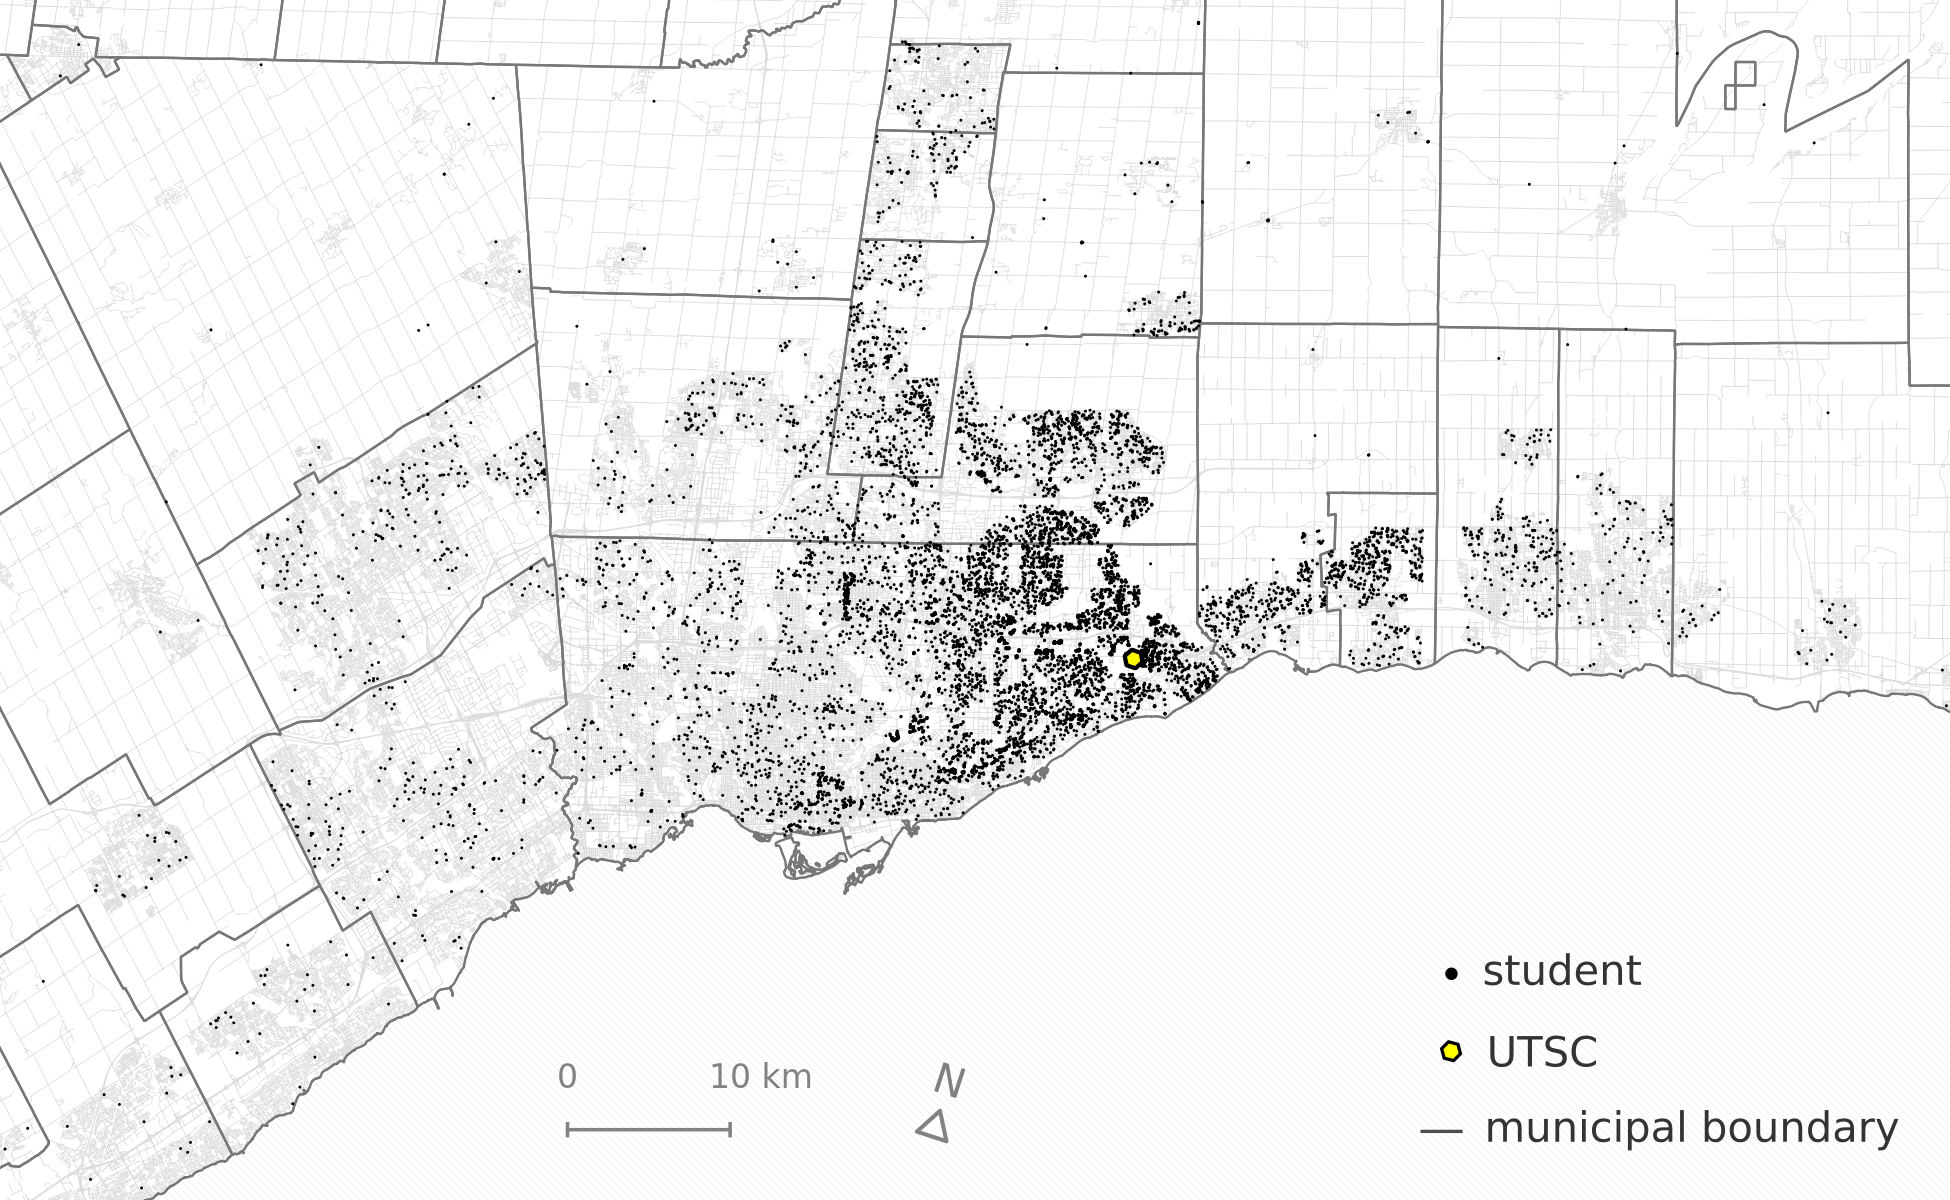
\includegraphics[width=5.5in]{figures/point_students.png}}
		\vspace{2mm}
	\end{figure}
	
	\begin{figure}[H]
		\vspace{2mm}
		\caption{Location of UTSC staff and faculty}
		\vspace{2mm}
		\label{pt_stafffaculty}
		\centerline{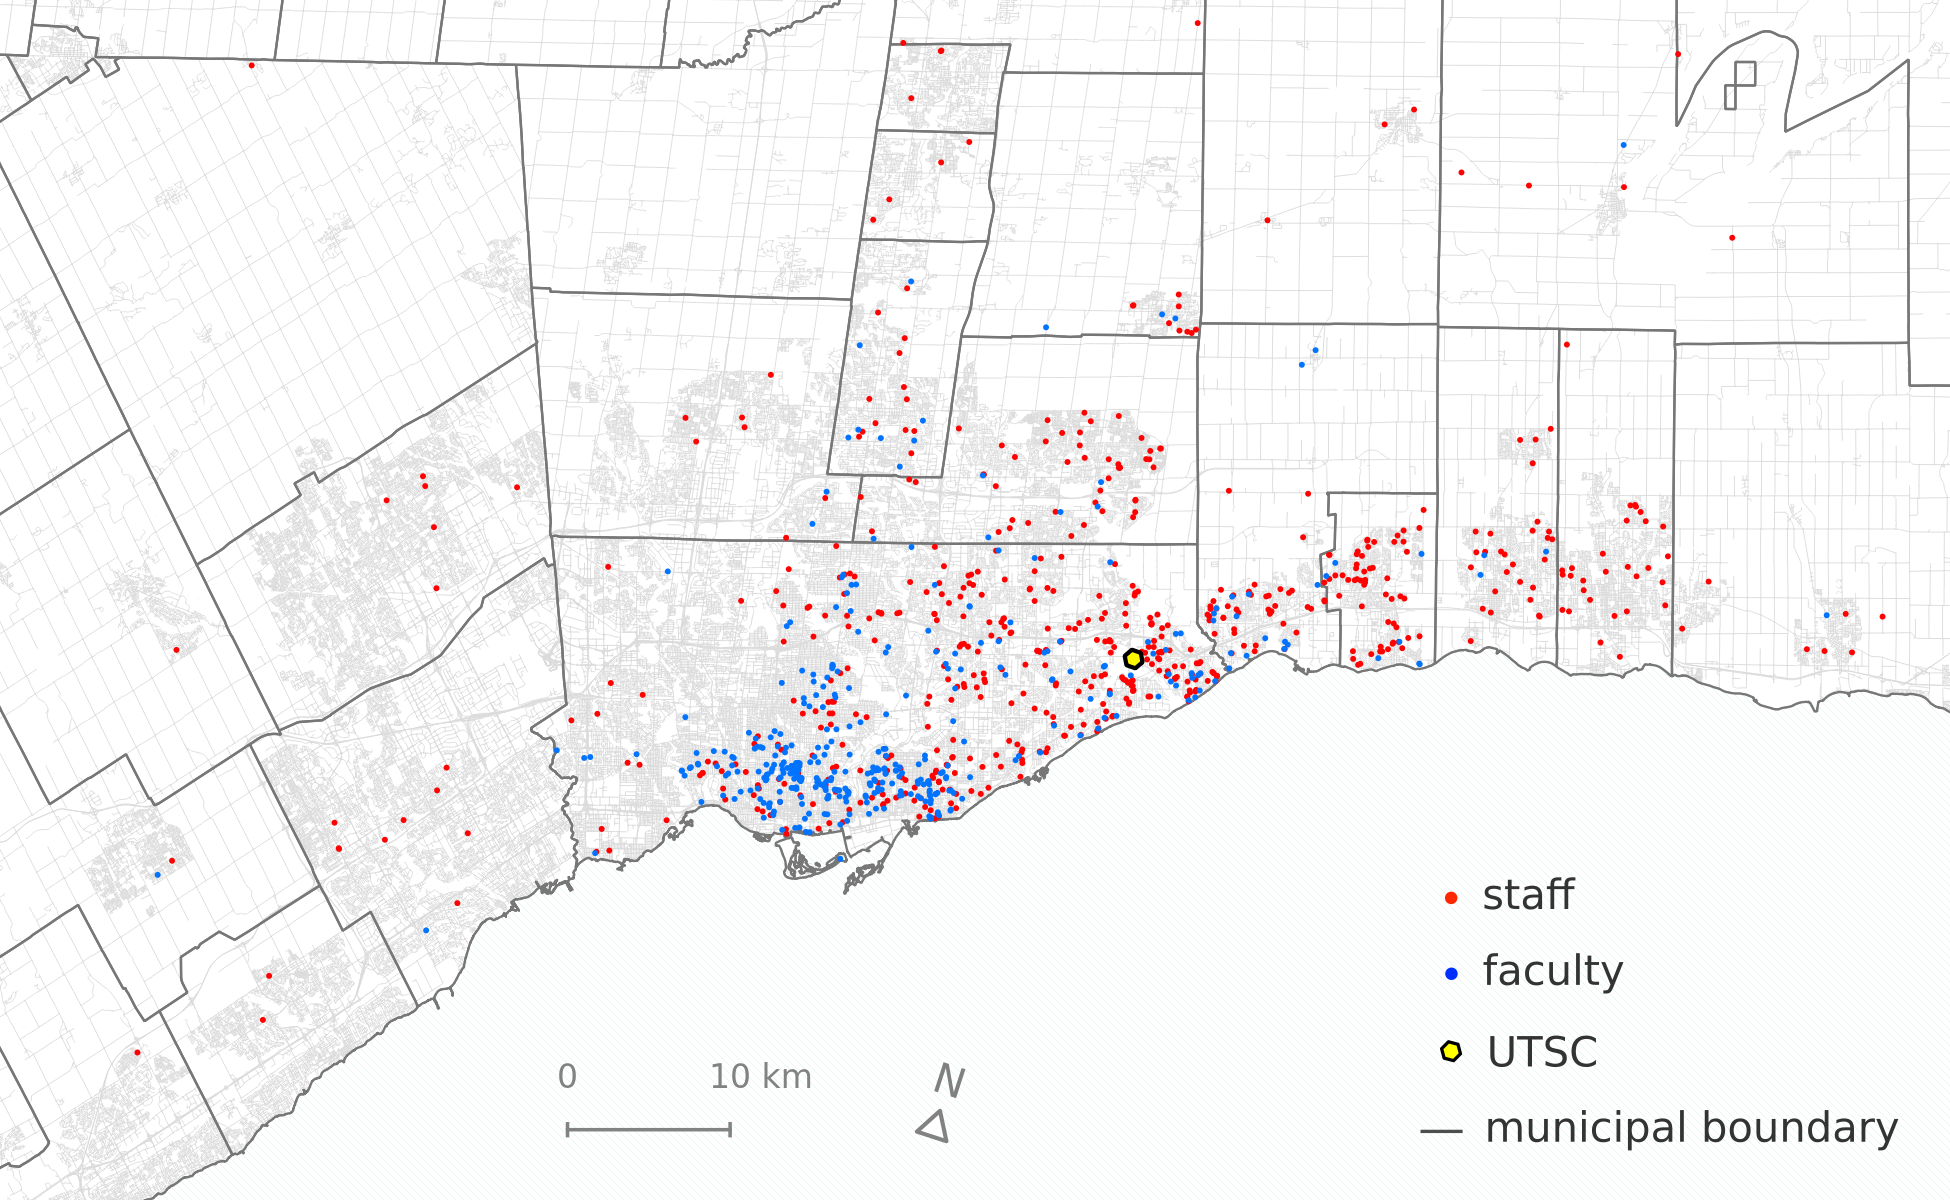
\includegraphics[width=5.5in]{figures/point_stafffaculty.png}}
		\vspace{2mm}
	\end{figure}


\section{Route maps and descriptions}\label{appendix:route_descriptions}

	The routes mentioned in Section \ref{sec:reliability} are described in detail here. Where possible, links to the relevant \href{http://www.openstreetmap.org}{OpenStreetMap} relation have been provided so the reader can see the route in the context of an interactive web map. 

	\textbf{Route 95} runs east-west along York Mills and Ellesemere Roads from York Mills Station at the western terminus to the UTSC campus or a little beyond. There are four variants of the route, described in Table \ref{t:route-variants}. 
	
	\textbf{Route 38} partly overlaps route 95 and runs along Ellesmere Road between Scarborough Town Centre and UTSC. There are two variants of the route. 
	
	\textbf{Route 198} runs express between Kennedy Station on Line 2 and the UTSC bus terminal. It travels along Eglinton, Kingston and Morningside and makes stops where transfers to another line are possible. 
	
	\textbf{Route 86} runs parallel to route 198 between Kennedy Station and Morningside Avenue. At Morningside it continues straight on Kingston Road whereas the 198 turns on Morningside. There are five variants of the route, only three of which are relevant and described in Table \ref{t:route-variants}.
	
	\begin{center}
		\begin{tabular}{ c | c | p{7cm} }
			\textbf{Route} & \textbf{Web map} & \textbf{Description} \\
			\hline
			198 & (\href{https://www.openstreetmap.org/relation/7906759}{east}, \href{https://www.openstreetmap.org/relation/8265811}{west}) & Runs express between Kennedy Station and the UTSC bus terminal making 12 intermediate stops. \\
			\hline
			86A & (\href{https://www.openstreetmap.org/relation/7890415}{both directions}) & Terminates at the Toronto Zoo \\
			\hline
			86B & (\href{https://www.openstreetmap.org/relation/7890416}{both directions}) & Terminates just past Military Trail\\
			\hline
			86C & (\href{https://www.openstreetmap.org/relation/283248}{both directions}) & Terminates at Sheppard and Meadowvale\\
			\hline
			95A & (\href{https://www.openstreetmap.org/relation/122331}{east}, \href{https://www.openstreetmap.org/relation/8265932}{west}) & Continues 3km east past UTSC on Ellesemere \\
			\hline
			95B & (\href{https://www.openstreetmap.org/relation/8267860}{east}, \href{https://www.openstreetmap.org/relation/8267859}{west}) & Runs local to the UTSC bus terminal. \\
			\hline
			95C & | & Does not extend as far as UTSC and is not considered here. \\
			\hline
			95E & (\href{https://www.openstreetmap.org/relation/8267989}{east}, \href{https://www.openstreetmap.org/relation/8267990}{west}) & Runs express to the UTSC bus terminal, making 18 intermediate stops. \\
			\hline
			38A & (\href{https://www.openstreetmap.org/relation/8265995}{east}, \href{https://www.openstreetmap.org/relation/90087}{west}) & Extends south-east past UTSC to the Rouge Hill GO station \\
			\hline
			38B & (\href{https://www.openstreetmap.org/relation/7886597}{east}, \href{https://www.openstreetmap.org/relation/8267814}{west}) & Stops at the UTSC bus terminal \\
		\end{tabular}
		\captionof{table}{Descriptions of bus lines mentioned in Section \ref{sec:reliability}.}
		\label{t:route-variants}
	\end{center}

%\section{Time and so on}
%
%\begin{center}
%	\begin{tabular}{c | l}
%		\textbf{Time period} & \textbf{Description} \\
%		\hline
%		7am - 9am & Morning Peak \\
%		9am - 4pm & Midday \\
%		4pm - 6pm  & Evening Peak \\
%		6pm - 10pm  & Evening \\
%	\end{tabular}
%	\captionof{table}{Weekday time periods.}
%	\label{t:timezones}
%\end{center} 



\printbibliography

\end{document}          
